\documentclass[a4paper,11pt,fleqn]{article}\usepackage[]{graphicx}\usepackage[]{color}
%% maxwidth is the original width if it is less than linewidth
%% otherwise use linewidth (to make sure the graphics do not exceed the margin)
\makeatletter
\def\maxwidth{ %
  \ifdim\Gin@nat@width>\linewidth
    \linewidth
  \else
    \Gin@nat@width
  \fi
}
\makeatother

\definecolor{fgcolor}{rgb}{0, 0, 0}
\newcommand{\hlnum}[1]{\textcolor[rgb]{0,0,0}{#1}}%
\newcommand{\hlstr}[1]{\textcolor[rgb]{0,0,0}{#1}}%
\newcommand{\hlcom}[1]{\textcolor[rgb]{0.4,0.4,0.4}{\textit{#1}}}%
\newcommand{\hlopt}[1]{\textcolor[rgb]{0,0,0}{\textbf{#1}}}%
\newcommand{\hlstd}[1]{\textcolor[rgb]{0,0,0}{#1}}%
\newcommand{\hlkwa}[1]{\textcolor[rgb]{0,0,0}{\textbf{#1}}}%
\newcommand{\hlkwb}[1]{\textcolor[rgb]{0,0,0}{\textbf{#1}}}%
\newcommand{\hlkwc}[1]{\textcolor[rgb]{0,0,0}{\textbf{#1}}}%
\newcommand{\hlkwd}[1]{\textcolor[rgb]{0,0,0}{\textbf{#1}}}%

\usepackage{framed}
\makeatletter
\newenvironment{kframe}{%
 \def\at@end@of@kframe{}%
 \ifinner\ifhmode%
  \def\at@end@of@kframe{\end{minipage}}%
  \begin{minipage}{\columnwidth}%
 \fi\fi%
 \def\FrameCommand##1{\hskip\@totalleftmargin \hskip-\fboxsep
 \colorbox{shadecolor}{##1}\hskip-\fboxsep
     % There is no \\@totalrightmargin, so:
     \hskip-\linewidth \hskip-\@totalleftmargin \hskip\columnwidth}%
 \MakeFramed {\advance\hsize-\width
   \@totalleftmargin\z@ \linewidth\hsize
   \@setminipage}}%
 {\par\unskip\endMakeFramed%
 \at@end@of@kframe}
\makeatother

\definecolor{shadecolor}{rgb}{.97, .97, .97}
\definecolor{messagecolor}{rgb}{0, 0, 0}
\definecolor{warningcolor}{rgb}{1, 0, 1}
\definecolor{errorcolor}{rgb}{1, 0, 0}
\newenvironment{knitrout}{}{} % an empty environment to be redefined in TeX

\usepackage{alltt}

%%----------------------------------------------------------------------
%% opções comuns
\usepackage[brazilian]{babel}
\usepackage[utf8]{inputenc}
\usepackage[T1]{fontenc}
\usepackage{textcomp}
%\usepackage[margin=2cm]{geometry}
\usepackage{indentfirst}
\usepackage{fancybox}
%\usepackage[usenames,dvipsnames]{color}
\usepackage{amsmath,amsfonts,amssymb,amsthm}
\usepackage{lscape}
\usepackage{natbib}
\setlength{\bibsep}{0.0pt}
\usepackage{url}
\usepackage{multicol}
\usepackage{multirow}
\usepackage[final]{pdfpages}
\usepackage{setspace}
\usepackage{paralist} % enumitem, compactitem
%%----------------------------------------------------------------------

%%----------------------------------------------------------------------
%% FLOATS: graficos e tabelas
\usepackage{graphicx}
\usepackage{float} % fornece a opção [H] para floats
\usepackage{longtable}
\usepackage{supertabular}
%% captions e headings em sans-serif
\usepackage[font={sf},labelfont={sf,bf}]{caption}
\usepackage{subcaption}
\renewcommand{\thesubfigure}{\Alph{subfigure}}
\usepackage{titlesec}
\titleformat*{\section}{\normalsize\bfseries\sffamily}
\titleformat*{\subsection}{\normalsize\bfseries\sffamily}
\titleformat*{\subsubsection}{\normalsize\bfseries\sffamily}
\titleformat*{\paragraph}{\normalsize\bfseries\sffamily}
\titleformat*{\subparagraph}{\normalsize\bfseries\sffamily}
\theoremstyle{definition}
\newtheorem*{mydef}{Definição}
%%----------------------------------------------------------------------

%%----------------------------------------------------------------------
%% definiçoes de hyperref e xcolor
\usepackage{hyperref}
\usepackage{xcolor}
%%----------------------------------------------------------------------

%%----------------------------------------------------------------------
%% FONTES

%% micro-tipografia
\usepackage[protrusion=true,expansion=true]{microtype}
%% Bitstream Charter with mathdesign
\usepackage{lmodern} % sans-serif: Latin Modern
\usepackage[charter]{mathdesign} % serif: Bitstream Charter
\usepackage[scaled]{beramono} % truetype: Bistream Vera Sans Mono
\usepackage[scaled]{helvet}
%\usepackage{inconsolata}


%\usepackage[sf]{titlesec}
%%----------------------------------------------------------------------

%%----------------------------------------------------------------------
%% hifenização
\usepackage[htt]{hyphenat} % permite hifenizar texttt. Ao inves disso
% pode usar \allowbreak no ponto qu quiser quebrar dentro do texttt
\hyphenation{con-si-de-ra-ção pes-que-i-ros pes-que-i-ra se-gui-do-ras
  di-fe-ren-tes pla-ni-lha pla-ni-lhão re-fe-ren-te con-ta-gem
  em-bar-ques qua-li-da-de a-le-a-to-ri-za-dos}
%%----------------------------------------------------------------------

%%----------------------------------------------------------------------
%% comandos customizados
\usepackage{xspace} % lida com os espaços depois dos comandos
\providecommand{\eg}{\textit{e.g.}\xspace}
\providecommand{\ie}{\textit{i.e.}\xspace}
\providecommand{\R}{\textsf{R}\xspace}
\newcommand{\mb}[1]{\mathbf{#1}}
\newcommand{\bs}[1]{\boldsymbol{#1}}
\providecommand{\E}{\text{E}}
\providecommand{\Var}{\text{Var}}
\providecommand{\logit}{\text{logit}}
%% Para alterar o titulo do thebibliography
\addto\captionsbrazilian{%
  \renewcommand{\refname}{Bibliografia}
}
%%----------------------------------------------------------------------

%%----------------------------------------------------------------------
%% Comandos para deixar o texto mais compacto
\usepackage{marginnote}
\usepackage[top=1cm, bottom=1cm, inner=1cm, outer=1cm,nohead, nofoot, heightrounded, marginparsep=.05cm]{geometry}
\setlength{\parindent}{0pt}
%%----------------------------------------------------------------------
\IfFileExists{upquote.sty}{\usepackage{upquote}}{}
\begin{document}

\reversemarginpar % para colocar a marginnote a esquerda





\hrule
\vspace{0.3cm}

\begin{minipage}[c]{.85\textwidth}
  Estatística II --- CE003 \\
  Prof. Fernando de Pol Mayer --- Departamento de Estatística --- DEST \\
  Exercícios: amostragem e análise exploratória de dados \\
  Nome: GABARITO  \hfill GRR: \hspace{2cm}
\end{minipage}\hfill
\begin{minipage}[c]{.15\textwidth}
\flushright

\includegraphics[width=2.2cm]{../img/ufpr-logo.png}
\end{minipage}

\vspace{0.3cm}
\hrule
\vspace{0.3cm}
%%----------------------------------------------------------------------

\begin{compactenum}[1.]
\item Estime as medidas de centro (média, mediana,
  moda) para amostras de altura de uma espécie de árvore (metros),
  coletadas em quatro áreas diferentes:
  \begin{itemize}
  \item[a)] Área A: 9,2 10,8 10,6 11,1 12,1 9,6 11,2 8,4 12,9 12,1
    14,4 11,1 11,1 9,7 8,4 12,3 10,7 12,9 9,1 12,8;
  \item[b)] Área B: 12,5 18,5 21,3 14,3 18,5 19,0 10,8 23,1 17,4 10,7
    14,3 16,3 18,0 7,1 12,8 14,7 11,3 8,2 13,8;
  \item[c)] Área C: 21,3 28,7 15,8 24,0 13,7 18,1 12,6 14,6 6,1 19,8
    22,3 15,7 16,3 18,2 15,7 6,6 9,3 1,3 19,0;
  \item[d)] Área D: 13,7 8,6 14,9 10,2 14,0 10,5 15,0 5,2 10,0 11,7
    18,7 9,3 7,9 6,5 11,5 12,0 8,3 8,3 9,8 4,7.
  \end{itemize}
\begin{knitrout}\small
\definecolor{shadecolor}{rgb}{1, 1, 1}\color{fgcolor}\begin{kframe}
\begin{verbatim}
$a
  media mediana    moda 
 11.025  11.100  11.100 

$b
   media  mediana    moda1    moda2 
14.87368 14.30000 14.30000 18.50000 

$c
   media  mediana     moda 
15.74211 15.80000 15.70000 

$d
  media mediana    moda 
  10.54   10.10    8.30 
\end{verbatim}
\end{kframe}
\end{knitrout}
\end{compactenum}

\vspace{0.3cm}
\hrule
\vspace{0.3cm}

\begin{compactenum}[2.]
\item Calcule a amplitude, a variância, o desvio-padrão, e o coeficiente
  de variação para as quatro amostras do exercício anterior.
\begin{knitrout}\small
\definecolor{shadecolor}{rgb}{1, 1, 1}\color{fgcolor}\begin{kframe}
\begin{verbatim}
              a         b         c         d
media 11.025000 14.873684 15.742105 10.540000
AMP    6.000000 16.000000 27.400000 14.000000
VAR    2.657763 18.556491 43.942573 12.318316
DP     1.630265  4.307725  6.628919  3.509746
CV    14.786982 28.962055 42.109485 33.299296
\end{verbatim}
\end{kframe}
\end{knitrout}
\end{compactenum}

\vspace{0.3cm}
\hrule
\vspace{0.3cm}

\begin{compactenum}[3.]
\item Descreva comparativamente as quatro áreas quanto à altura das
  árvores, utilizando as estatísticas que você calculou.\\
  (\textit{Exemplo de resposta}) Em média, a área C possui as árvores
  mais altas ($\bar{x}_C = 14,874$), enquanto que a área D possui as
  árvores mais baixas ($\bar{x}_D = 10,54$). Em todas as áreas, o valor
  da mediana está muito próximo do valor da média e da moda, o que
  indica que a distribuição das alturas em todas as áreas é
  aproximadamente simétrica. A maior amplitude de variação de alturas
  foi observada na área C, que também apresentou a maior variabilidade
  das observações em relação à média, como pode ser observado pelos
  valores da variância ($s^2_C = 43,943$), e do desvio-padrão ($s_C =
  6,629$). A área com árvores de alturas mais homogêneas foi a A, pois a
  amplitude foi de 6 m, e a varibilidade das alturas em torno da média
  foi a menor quando comparada com as demais áreas ($s^2_A = 2,658$ e
  $s_A = 1,63$). Estas diferenças de variabilidade podem ser observadas
  através do coeficiente de variação, que foi de 42,1\% para a área C, e
  de 14,8\% para a área A. A área D apresentou um CV de 33,3\%, enquanto
  que o CV da área B foi de 28,9\%.
\end{compactenum}

\vspace{0.3cm}
\hrule
\vspace{0.3cm}

%% \begin{compactenum}[4.]
%% \item Calcule os escores z para todos os elementos das amostras das
%%   áreas A e C dadas no exercício 2. Identifique se há valores não
%%   usuais. Justifique. Explique o que significa os valores de escore $z$
%%   ou escore padronizado.
%% <<echo=-c(3,4)>>=
%% ## Escores Z calculados na ordem que os dados estão  apresentados
%% (zs <- apply(ex2[, c(1,3)], 2, z))
%% za <- as.vector(zs[,1])
%% zc <- as.vector(zs[,2])
%% ## Valores de Z não usuais
%% za[za < -2 | za > 2]
%% zc[zc < -2 | zc > 2]
%% ## Referentes aos respectivos valores de x
%% a[which(za < -2 | za > 2)]
%% c[which(zc < -2 | zc > 2)]
%% @
%% \end{compactenum}

%% \vspace{0.3cm}
%% \hrule
%% \vspace{0.3cm}

\begin{compactenum}[5.] % magalhaes, pg 30
\item Um exame vestibular para uma faculdade tem 80 questões, sendo 40
  de português e 40 de matemática. Para os 20 melhores classificados,
  apresentamos o número de acertos em cada disciplina.
  \begin{itemize}
  \item Português: 35, 35, 34, 32, 31, 30, 26, 26, 24, 23, 23, 12, 11,
    20, 17, 12, 14, 20, 8, 10
  \item Matemática: 31, 29, 27, 28, 28, 26, 30, 28, 25, 23, 21, 32, 31,
    20, 21, 25, 20, 13, 23, 20
  \end{itemize}

\begin{compactenum}
\item Calcule as medidas de centro: média, mediana e moda para cada grupo
\begin{knitrout}\small
\definecolor{shadecolor}{rgb}{1, 1, 1}\color{fgcolor}\begin{kframe}
\begin{verbatim}
$port
  media mediana   moda1   moda2   moda3   moda4   moda5 
  22.15   23.00   12.00   20.00   23.00   26.00   35.00 

$mat
  media mediana   moda1   moda2 
  25.05   25.50   20.00   28.00 
\end{verbatim}
\end{kframe}
\end{knitrout}
  \item Calcule as medidas de variabilidade: variância, desvio-padrão, e
    coeficiente de variação para cada grupo
\begin{knitrout}\small
\definecolor{shadecolor}{rgb}{1, 1, 1}\color{fgcolor}\begin{kframe}
\begin{verbatim}
         port       mat
VAR 80.134211 23.839474
DP   8.951771  4.882568
CV  40.414318 19.491291
\end{verbatim}
\end{kframe}
\end{knitrout}
  \item Calcule o resumo dos cinco números para cada grupo
\begin{knitrout}\small
\definecolor{shadecolor}{rgb}{1, 1, 1}\color{fgcolor}\begin{kframe}
\begin{verbatim}
    port  mat
Min  8.0 13.0
Q1  13.0 21.0
Q2  23.0 25.5
Q3  30.5 28.5
Max 35.0 32.0
\end{verbatim}
\end{kframe}
\end{knitrout}
  \item Construa um gráfico de caixa para cada grupo (em um mesmo
    gráfico para comparação)
\begin{knitrout}\small
\definecolor{shadecolor}{rgb}{1, 1, 1}\color{fgcolor}

{\centering 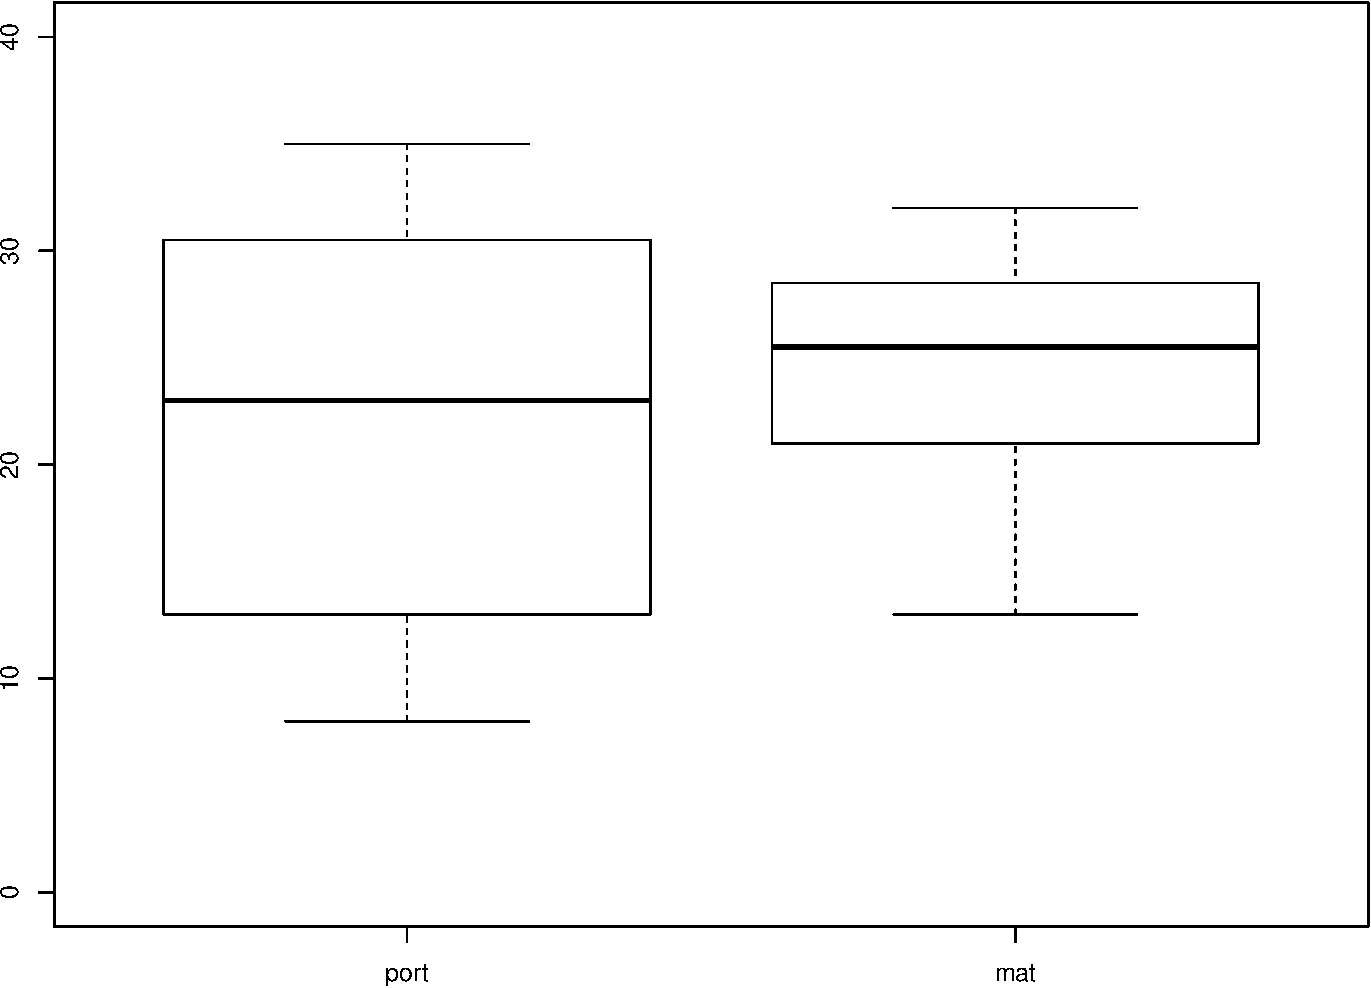
\includegraphics[width=.5\textwidth]{figure/unnamed-chunk-7-1} 

}



\end{knitrout}

\item Com todos os resultados obtidos, descreve comparativamente estes
    dois grupos em termos de medidas de tendência central,
    variabilidade, amplitude e distribuição (simetria) dos dados.\\
    (\textit{Exemplo de resposta}) Em média, o número de acertos em
    matemática ($\bar{x}_{mat} = 25,05$) foi maior do que o número de
    acertos em português ($\bar{x}_{port} = 22,15$). A diferença entre
    os valores médios e a mediana mostra que existe uma leve assimetria
    negativa (ou à esquerda) para os dois casos ($\bar{x} < \text{Me}$),
    embora esta diferença seja mais pronunciada nas notas de
    português. A amplitude do número de acertos em português foi de
    $\text{AMP}_{port} = 35-8=27$, maior do que a amplitude obervada
    para o número de acertos em matemática, que foi de
    $\text{AMP}_{port} = 32-13=19$. A variabilidade dos acertos em torno
    da média também foi maior para as notas de português, com variância
    de $s^2_{port} = 80,134$ e desvio-padrão de $s_{port} = 8,951$. Já
    para a matemátiva, a variabilidade em torno da média foi menor, com
    $s^2_{mat} = 23,839$ e desvio-padrão $s_{mat} = 4,883$. Resumindo
    estas informações sobre variabilidade, nota-se que o coeficiente de
    variação para português foi de 40,4\%, enquanto que para a
    matemática foi menor, com aproximadamente 19,5\%. Através do resumo
    dos cinco números e do gráfico de caixa, percebe-se que 50\% dos
    acertos foram entre 13 e 30,5 em português (diferença entre Q1 e
    Q3), e entre 21 e 28,5 em matemática, mostrando novamente a menor
    variabilidade observada para a matemática.
  \item Você acha que os aprovados são melhores em português ou
    matemática?
  \end{compactenum}
\end{compactenum}

%% \vspace{0.3cm}
%% \hrule
%% \vspace{0.3cm}

%% \clearpage

\vspace{0.3cm}
\hrule
\vspace{0.3cm}

\begin{compactenum}[6.] % magalhaes, pg 31
\item Deseja-se comparar três técnicas cirúrgicas para a extração do
  dente siso. Cada uma das técnicas foi aplicada a 30 pacientes, e os
  resultados são apresentados em diagramas de caixa abaixo.\vspace{1em}
\begin{knitrout}\small
\definecolor{shadecolor}{rgb}{1, 1, 1}\color{fgcolor}

{\centering 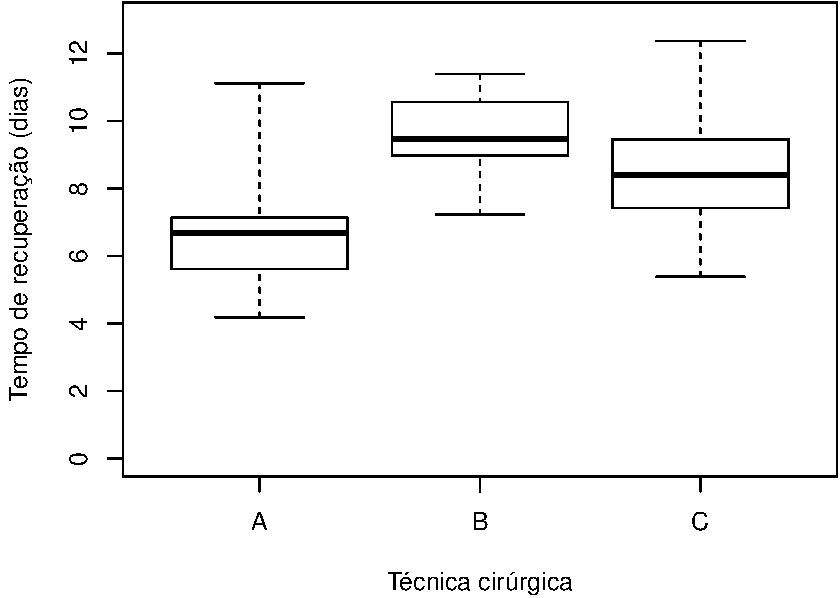
\includegraphics[width=.5\textwidth]{figure/siso-1} 

}



\end{knitrout}
\begin{compactenum}
\item Encontre os valores (aproximados) para a mediana, os quartis,
  máximo e mínimo.
\begin{knitrout}\small
\definecolor{shadecolor}{rgb}{1, 1, 1}\color{fgcolor}\begin{kframe}
\begin{alltt}
\hlcom{## Estes são os valores exatos!}
\end{alltt}
\begin{verbatim}
            A         B         C
Min  4.184541  7.228075  5.388393
Q1   5.623099  8.977717  7.430463
Q2   6.686161  9.476333  8.410870
Q3   7.137260 10.565402  9.456991
Max 11.120594 11.397466 12.372938
\end{verbatim}
\end{kframe}
\end{knitrout}
\item Discuta a variabilidade do tempo de recuperação em cada técnica. \\
  (\textit{Exemplo de resposta}) A amplitude de dias de recuperação para
  as técnicas A, B, e C, são, respectivamente: $\text{AMP}_{A} = 11,121
  - 4,185 = 6,936$, $\text{AMP}_{B} = 11,398 - 7,228 = 4,17$,
  $\text{AMP}_{C} = 12,373 - 5,388 = 6,985$. Com isso, percebe-se que a
  técnica A apresenta um tempo de recuperação (aproximado) entre 4 e 11
  dias, a técnica B entre 7 e 11 dias, e a técnica C entre 5 e 12
  dias. A maior variação de tempo de recuperação foi então da técnica C
  (maior amplitude), enquanto que a técnica B apresentou a menor
  variação. Nota-se, em termos de mediana, que a técnica A apresentou o
  menor tempo de recuperação (Me = 6,69), embora com uma grande
  variabilidade. Além disso, percebe-se através do gráfico de caixa, que
  a técnica A possui uma distribuição com assimetria positiva, como pode
  ser observado pela proximidade da mediana com o terceiro quuartil
  (Q3), além de uma extensão maior da caixa até o valor máximo. A
  técnica B apresentou um tempo de recuperação mediano de 9,47 dias, o
  maior observado entre as 3 técnicas. Percebe-se também que a
  distribuição do tempo de recuperação para esta técnica é levemente
  assimétrica à esquerda, pois a mediana está deslocada para baixo
  dentro da caixa. O tempo de recuperação mediano para a técnica C foi
  de 8,41 dias. Para esta técnica, 50\% das pessoas tiveram um tempo de
  recuperação entre 7,43 (Q1) e 9,46 (Q3) dias.
\item Se você é otimista, qual técnica escolheria?
\end{compactenum}
\end{compactenum}

\vspace{0.3cm}
\hrule
\vspace{0.3cm}

\begin{compactenum}[7.] % vieira, pg 64
\item A distribuição das estaturas, em centímetros, de alunos de um
  curso colegial está representada na tabela de frequência abaixo.
  %% \begin{table}[h]
  %%   \centering
  %%   \begin{tabular}{cr}
  %%     \hline
  %%     \textbf{Classes} & \textbf{Frequência} \\
  %%     \hline
  %%     $135 \vdash 145$ & 15 \\
  %%     $145 \vdash 155$ & 150 \\
  %%     $155 \vdash 165$ & 250 \\
  %%     $165 \vdash 175$ & 70 \\
  %%     $175 \vdash 185$ & 10 \\
  %%     $185 \vdash 195$ & 5 \\
  %%     \hline
  %%   \end{tabular}
  %% \end{table}
  Calcule a média, a variância, e o desvio-padrão das estaturas.
  \begin{table}[htbp]
    \begin{center}
      \begin{tabular}{cccccc}
        \hline
        Classes          & Frequência & PM = $X_i$ & $X_if_i$ & $X_i^2$ & $X_i^2f_i$ \\
        \hline
        $135 \vdash 145$ & 15         & 140        & 2100     & 19600   & 294000     \\
        $145 \vdash 155$ & 150        & 150        & 22500    & 22500   & 3375000    \\
        $155 \vdash 165$ & 250        & 160        & 40000    & 25600   & 6400000    \\
        $165 \vdash 175$ & 70         & 170        & 11900    & 28900   & 2023000    \\
        $175 \vdash 185$ & 10         & 180        & 1800     & 32400   & 324000     \\
        $185 \vdash 195$ & 5          & 190        & 950      & 36100   & 180500     \\
        \hline
        Total            & 500        &            & 79250    &         & 12596500   \\
        \hline
      \end{tabular}
    \end{center}
  \end{table}



\begin{align*}
  \bar{X} &= \frac{1}{n} \sum_{i=1}^{n} X_i f_i \\
  &= \frac{1}{500} \cdot 79250 \\
          &= 158,5
\end{align*}

\begin{align*}
  s^2 &= \frac{1}{n-1} \left[ \sum_{i=1}^{n} X_{i}^{2} f_i -
    \frac{(\sum_{i=1}^{n} X_{i} f_i)^2}{n} \right] \\
  &= \frac{1}{500-1} \left[ 12596500 - \frac{(79250)^2}{500} \right] \\
  &= 70,892
\end{align*}

\begin{align*}
  s &= \sqrt{70,892} \\
    &= 8,419
\end{align*}

\end{compactenum}

\vspace{0.3cm}
\hrule
\vspace{0.3cm}

\end{document}
